\chapter{OPERACIONES PCE}

\section{Introducción} % {{{
%\cpnote{Porfa tambien esqueleto de la into}
%\esqueleto{ 
%\begin{itemize}
%\item Hablar que es importante estudiar problemas de muchas 
%partículas.
%\item Con la teoría de los canales cuánticos se pueden estudiar una 
%gran variedad de sistemas, siendo uno de ellos los de sistemas de qubits.
%\item Hablar qué son los qubits: sistemas cuánticos de dos niveles. 
%\cpnote{Creo que es un poco tarde para hablar de qubits. Ya mencionaste las matrices
%de Pauli, y sería buen momento antes, o de plano no decir nada.}
%\item Escribir sobre la estructura del capítulo.
%\end{itemize}
%}
%
%\esqueleto{
%\hrule\vspace{10pt}
%\h{Párrafos}
%\begin{itemize}
%\item Los sistemas cuánticos de dos niveles han sido y siguen 
%siendo de gran importancia teórica y práctica para la mecánica 
%cuántica y sus aplicaciones.
%\item La teoría de los canales cuánticos se puede utilizar para estudiar 
%la dinámica de un gran variedad de sistemas cuánticos abiertos, pero el objetivo
%de este proyecto está centrado en el estudio de los canales cuánticos de qubits.
%\item La estructura del capítulo.
%\end{itemize}
%}
%
%El tipo de operaciones que estudiamos en este trabajo son operaciones 
%que actúan sobre sistemas de qubits. Un qubit es un sistema cuántico 
%de dos niveles \janote{cita}, como una partícula de espín 1/2. Los 
%canales cuánticos de 1 qubit son especialmente útiles para ganar intuición
%sobre los canales cuánticos ya que los estados de 1 qubit se 
%pueden representar geométricamente en la esfera de Bloch \janote{cita}.
%Los estados de 1 qubit en la esfera de Bloch se pueden relacionar con 
%su matriz de densidad al escribir esta en la base de las matrices 
%de Pauli como 
%\begin{align}
%\rho=\frac{1}{2}\sum_{i=0}^3r_i\sigma_i
%\end{align}

\janote{La intro la dejo para cuando termine de escribir el capítulo.}

% }}}
\section{Operaciones PCE} % {{{
%\esqueleto{
%Dos o tres párrafos máximo hablando sobre las operaciones PCE 
%como operaciones proyectivas a la base de productos tensoriales de 
%las matrices de Pauli. Me gustaría poner un problema de motivación
%sólo para hacer más interesante la lectura a partir de acá y dejarle al
%lector algo con lo que pueda entender qué onda con las operaciones 
%PCE. Propongo lo siguiente: cadena de espines. Supongamos una 
%cadena de espines de $N$ sitios y decimos que nos interesa saber 
%si la matriz de densidad del $i$-ésimo espín puede proyectarse 
%al subespacio cuya base son $\sigma_x$ y $\sigma_y$ (lo que 
%quiero decir es que $(r_x,r_y,r_z)\to(r_x,r_y,0)$). Entonces hablo 
%de que hay que considerar que el $i$-ésimo espín puede estar 
%entrelazado con el resto de la cadena, sin embargo, basta con considerar
%que se encuentra entrelazado con cualquiera de sus vecinos y revisar 
%en qué se transforma la matriz de densidad de esos dos espines para 
%averiguar si es posible tal evolución física. Me gustaría poner unas 
%figuritas para hacer interesante esto. 
%}

\esqueleto{La idea central de esta sección será: No todas las operaciones que 
borran componentes de Pauli de la matriz de densidad de 1 qubit no 
son canales cuánticos.}

\esqueleto{Introducir los canales cuánticos de 1 qubit 
de bit-flip y defasing como una motivación para definir qué es una 
operación PCE. Figuritas para la interpretación geométrica y discutir 
especialmente cómo actúan sobre las componentes de Pauli.}

\esqueleto{Mencionar los casos del bit-flip y defasing
cuando la esfera de Bloch se mapea a una linea sobre los ejes $x$ y $y$,
respectivamente. Nada nuevo, evidentemente son canales porque son 
casos particulares de otros que son canales. Introducir el punto de vista
de esos canales como operaciones que borran componentes.}

\esqueleto{Conducir al lector a preguntarse: `bueno, entonces deplano
que puedo borrar cualquier cantidad de componentes de Pauli, ¿no? ¡¿NO?!', 
pero nel. Recordar que vimos en el capítulo anterior la operación que 
mapea la esfera de Bloch a un disco sobre el plano $x$-$y$ y no es 
un canal cuántico... porque no es CP. Es decir, la condición de completa 
positividad es la que impide que las operaciones que borran componentes 
de Pauli de 1 qubit sean trivialmente canales cuánticos. Siempre será bueno
que dedique al menos una frase a recordar la implicación física de la CP: 
existe por lo menos un estado entrelazado en el espacio de 2 qubits 
que se mapea a un no estado.}

\esqueleto{Motivar a pensar que si la CP ya impide que algunas 
operaciones que borran componentes de Pauli de 1 qubit no sean
canales cuánticos entonces ¿qué ocurrirá en sistemas de más qubits 
que ya aparecen correlaciones cuánticas? (porque en el caso de 1 qubit 
la regla de $2^k$ es necesaria y suficiente, para más qubits también 
va a importar cuáles componentes se borran y en este punto debería 
ser una pregunta importante para quien no sepa la respuesta)}

\esqueleto{Ya, no más rodeos y finiquitar con la expresión de $\rho$ para 
$n$ qubits en la base de Pauli y definir formalmente una operación PCE.}


%
%\esqueleto{Ideas: \begin{itemize}
%\item Aprovechar que en el capítulo anterior hablé sobre la operación 
%que mapea la esfera de Bloch a un disco.
%\item Introducir el bit-flip y defasing.
%\end{itemize}}
%
%\cpnote{Siento qe aun no es un esqueleto sino ideas. De la motivación
%no me gusta como la abordas. Yo pensaría mejor en hablar un poco de defasing
%y de bitflip para uno y muchos qubits. Siento qeu tu propuesta está
%aun un poco por fuera de tu alcance y te propondría mantenerla más simple.
%Si quieres iteremos la propuesta, y cuando nos pongamos de acuerdo ya haces un esqueleto 
%mas a nivel de parrafos.}
%
%\esqueleto{
%\begin{itemize}
%\item Para introducir el contexto de las operaciones PCE voy mencionar sobre
%el defasing y el bitflip channel cuando $p=0.5$.
%\item Luego hablar sobre
%la extensión de este tipo de canales cuánticos para sistemas de 2 
%qubits. Mencionar que es intuitivo entender que localmente, sobre cada qubit,  
%las únicas evoluciones físicas son las que ya se conocen para 1 qubit 
%(bitflip, defasing y bit-phase flip).
%\item Sin embargo, el problema cobra interés
%al considerar que el estado de 2 qubits es más que 
%sólo la suma del estado del qubit 1 y del qubit 2, ya que aparecen 
%las correlaciones cuánticas.
%\item Mencionar que 
%vamos a entender a este tipo de canales cuánticos como operaciones 
%que `borran' las componentes del vector de Bloch generalizado de un 
%sistema de qubits.
%\item Por último, mencionar que 
%el entrelazamiento en sistemas de muchas partículas nos conduce
%a preguntarnos de qué forma puede un canal cuántico las correlaciones
%cuánticas de un sistema de qubits.
%\end{itemize}
%}


%\esqueleto{
%\hrule \vspace{10pt}
%\h{Párrafos}
%\begin{itemize}
%\item El defasing y bitflip channel cuando $p=0.5$ se pueden entender 
%como canales cuánticos de 1 qubit que borran 2 componentes del 
%vector de Bloch y a la componente restante la dejan invariante.
%¿Cómo son los canales cuánticos de este tipo, 
%que borran las componentes del vector de Bloch, para 2 qubits?
%\item Por la matriz de densidad reducida las evoluciones permitidas 
%localmente sobre cada qubit son defasing, bitflip y bit-phase fip.
%\item Al examinar la matriz de densidad para 2 qubits
%se puede distinguir que está compuesta por componentes locales 
%de cada qubit + correlaciones entre ambas partículas. 
%Esto conduce principalmente a la pregunta 
%¿de qué forma se pueden borrar las correlaciones cuánticas tal que 
%esa evolución sea física?
%\item Recursivamente, al aumentar el número de partículas en 
%el sistema, aparecen nuevas correlaciones que no sabemos de 
%qué manera se pueden borrar para que ese proceso cumpla con
%las condiciones para ser una evolución que físicamente pueda ocurrir.
%El `borrado' está condicionado por la completa positividad que 
%debe de satisfacer la operación.
%\end{itemize}
%}

%%%%%%%%%%%%%%%%%%%%%%%%%%%%%%%%
%% Esto podría servir
%%%%%%%%%%%%%%%%%%%%%%%%%%%%%%%%

%Para establecer qué son las operaciones PCE y el porqué de nuestro interés por 
%estudiarlas vamos a hablar antes de dos ejemplos 
%de canales cuánticos de 1 qubit. Estos dos ejemplos junto con la operación
%$\E_z$, que discutimos en la sección \ref{sec:qtm-channels}, nos servirán 
%como punto de partida para motivar el estudio de un tipo muy particular 
%de operaciones, que actúan sobre sistemas de qubits, a los cuáles hemos
%bautizado con el nombre de operaciones de Pauli que borran 
%componentes (PCE por sus siglas en inglés, \textit{Pauli component erasing}).
%
%Los canales cuánticos de 1 qubit que discutiremos son el canal 
%de inversión de bit y el canal de inversión de fase. 
%Geométricamente, ambos canales deforman la bola 
%de Bloch en un elipsoide con eje de simetría en $x$ y $y$,
%respectivamente (Figs. \ref{fig:bit-flip} y \ref{fig:phase-flip}).
%Los semiejes perpendiculares al eje de simetría del elipsoide
%varían según un parámetro $p$. Especifícamente
%nos interesa revisar el caso de los canales de inversión de bit 
%y de inversión de fase cuando la bola de Bloch se mapea a una 
%línea sobre el eje de simetría del elipsoide.
%
%Recordemos que la matriz de densidad de 1 qubit
%se escribe en la base de matrices de Pauli
%como $\rho^1$ en %\eqref{eq:densityMatrices_1and2Qubits}.
%El canal cuántico de inversión de bit transforma a las componentes 
%$r_i$ de $\rho^1$ como $(1,r_x,r_y,r_z)\to\qty(1,r_x,(1-2p)r_y,(1-2p)r_z)$, 
%con $p$ un parámetro que se encuentra entre 0 y 1.
%Cuando $p=0.5$, el canal inversor de bit hace cero las 
%componentes $r_y$ y $r_z$ de $\rho^1$. Geométricamente,
%mapea la bola de Bloch a una línea sobre el eje $x$.
%Decimos que el canal `borró' las componentes $r_y$ y $r_z$ de $\rho^1$. 
%De manera similar, cuando $p=0.5$, el canal 
%de inversión de fase `borra' las componentes $r_x$ y $r_y$
%de $\rho^1$ y mapea la bola de Bloch a una línea sobre el eje $z$.
%
%\begin{figure}
%\centering
%\begin{minipage}{.4\textwidth}
%    \centering
%    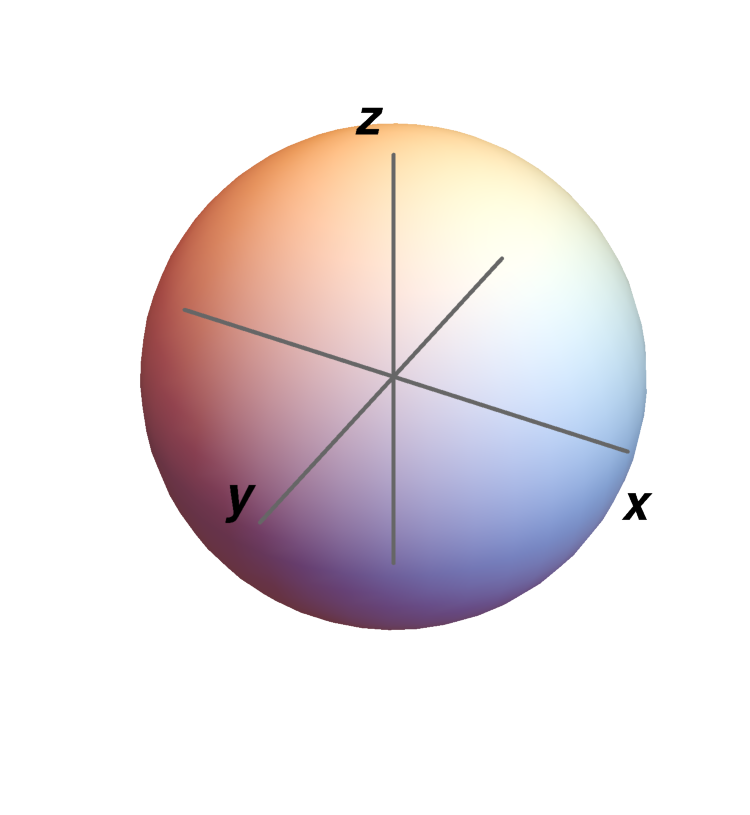
\includegraphics[width=4.5cm]{bloch-ball}
%\end{minipage}
%$\longmapsto$
%\begin{minipage}{0.4\textwidth}
%    \centering
%    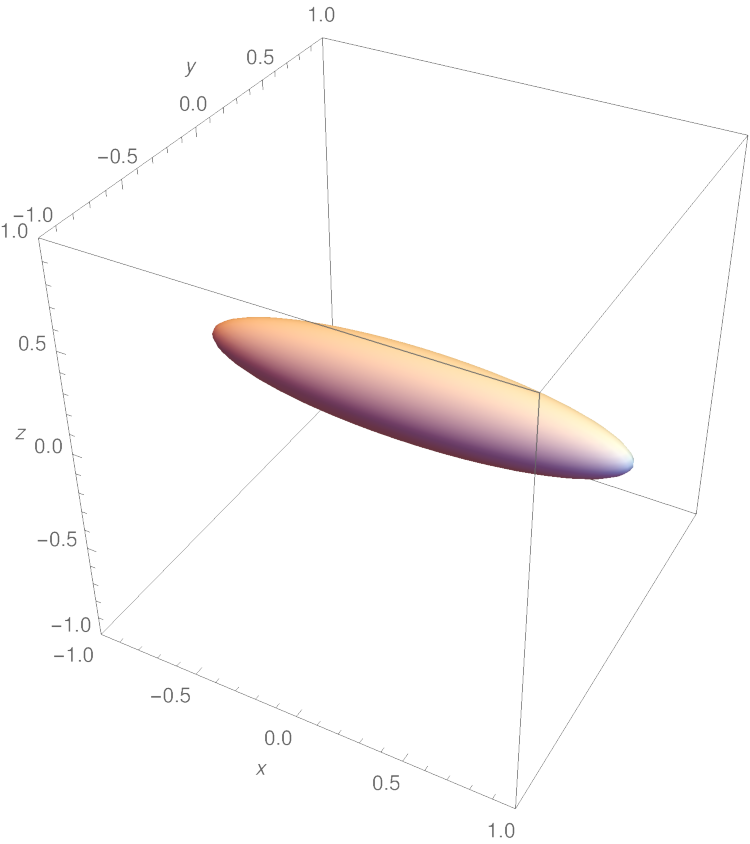
\includegraphics[width=4.5cm]{bit-flip}
%\end{minipage}
%\caption{
%Efecto del canal de inversión de bit sobre la esfera de Bloch, para $p=0.3$.}
%\label{fig:bit-flip}
%\end{figure}
%
%\begin{figure}
%\centering
%\begin{minipage}{.4\textwidth}
%    \centering
%    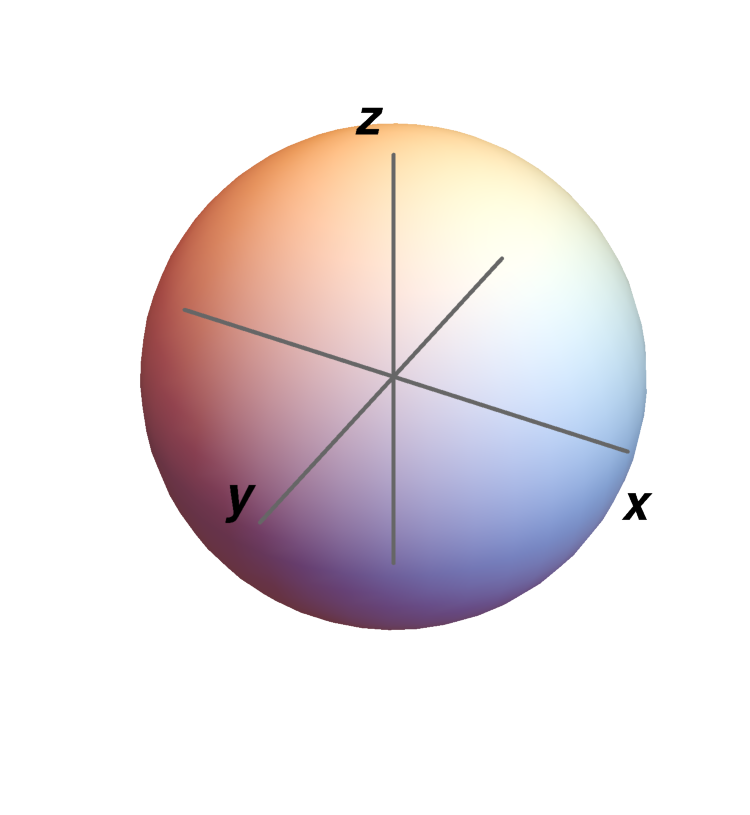
\includegraphics[width=4.5cm]{bloch-ball}
%\end{minipage}
%$\longmapsto$
%\begin{minipage}{0.4\textwidth}
%    \centering
%    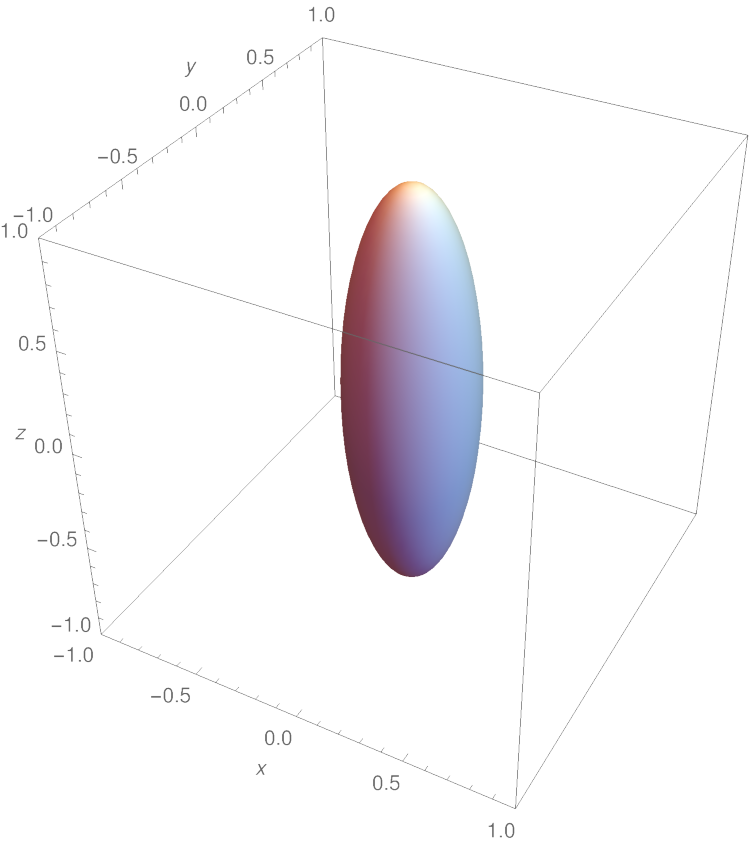
\includegraphics[width=4.5cm]{phase-flip}
%\end{minipage}
%\caption{
%Efecto del canal de inversión de bit sobre la esfera de Bloch, para $p=0.3$.}
%\label{fig:phase-flip}
%\end{figure}
%
%Por otro lado recordemos, de la sección \ref{sec:qtm-channels}, 
%que la operación $\E_z$, que borra la componente $r_z$ de $\rho^1$,
%no es un canal cuántico porque no satisface la condición de completa
%positivad. Esto significa que existe al menos un estado entrelazado en 
%el espacio extendido de 2 qubits que es mapeado por $\E_z\otimes \1$ 
%a una matriz que no es un estado físico de 2 qubits. 
%
%Recapitulando, revisamos tres ejemplos de operaciones que borran 
%componentes de la matriz de densidad de 1 qubit, escrita en la base 
%de matrices de Pauli. Dos de ellas satisfacen las condiciones para 
%ser canales cuánticos y una de ellas no porque no es una operación 
%completamente positiva. En otras palabras, las operaciones que 
%borran las componentes de Pauli de la matriz de densiad de 1 qubit 
%no satisfacen trivialmente las condiciones para ser canales cuánticos.
%Es así como nos preguntamos ¿cuáles son las características que
%comparten los canales cuánticos de 1 qubit que borran las componentes 
%de Pauli? 
%
%Estamos listos para formular la definición de las operaciones PCE y 
%cuál es el problema de nuestro interés. La matriz de densidad de $n$
%qubits puede escribirse en la base de los productos tensoriales 
%de las matrices de Pauli como
%\begin{align}\label{eq:rho-pauliBasis}
%\rho=\frac{1}{2^n}\sum_{j_1,\ldots,j_n=0}^3
%r_{j_1,\ldots,j_n}\sigma_{j_1}\ot \ldots\ot \sigma_{j_n},
%\end{align}
%donde $r_{j_1,\ldots,r_n}/2^n$ son las proyecciones de $\rho$ sobre 
%cada uno de los elementos $\sigma_{j_1}\ot \ldots\ot \sigma_{j_n}$. 
%Definimos entonces a una operación de Pauli que borra componentes (PCE)  
%como una operación que actúa sobre una matriz de densidad de $n$ qubits 
%de la forma \eqref{eq:rho-pauliBasis} haciendo cero a algún subconjunto
%de componentes $r_{j_1,\ldots,j_n}$ y dejando invariante al resto.
%El problema que nos planteamos es el de caracterizar a las operaciones 
%PCE que satisfacen la condición de completa positividad para ser 
%canales cuánticos. En las siguientes dos secciones vamos a profundizar
%en las operaciones PCE de 1 qubit y establecer la ruta a seguir para
%resolver el problema de un sistema de $n$ qubits.

%%%%%%%%%%%%%%%%%%%%%%%%%%%%%%%%
%%%%%%%%%%%%%%%%%%%%%%%%%%%%%%%%


% }}}
\section{1 qubit} % {{{
\esqueleto{
Idea central de esta sección: encontrar todos los canales cuánticos PCE 
de 1 qubit.}

\esqueleto{
Para resolver el problema lo que haremos será encontrar los eigenvalores 
de la matriz de Choi del superoperador y así encontrar las condiciones 
que debe satisfacer una operación PCE de 1 qubit para ser un canal cuántico
en términos de las $\tau_i$. 
Escribir al superoperador, en su forma diagonal con las $\tau_i$, 
que actúa sobre la matriz de densidad de 1 qubit escrita en la base de Pauli. 
}

\esqueleto{
Aplicar el reshuffle para encontrar la matriz de Choi y calcular después 
sus eigenvalores.
}

\esqueleto{
Enunciar las desigualdades que deben satisfacer las $\tau_i$ para que 
la operación sea un canal cuántico. Hacer referencia al resultado del
Geometry of Quantum States en el que también llegan a esas desigualdades
(tienen un nombre). Esto para hacerlo ver como un check de que no 
estamos hablando paja aquí.
}

\esqueleto{
Escribir las 8 operaciones PCE de 1 qubit y discutir sobre las operaciones 
que sí satisfacen las desigualdades para ser canales cuánticos y las que no.
Discutir que no hay nada fundalmente diferente entre las 3 operaciones
que mapean la esfera de Bloch a una línea, igual que las 3 que mapean 
la esfera de Bloch a un disco. Esto implica que hay una equivalencia
entre esas operaciones. 
Y fin. En conclusión, son canales cuánticos PCE solo los que dejan igual 
la esfera de Bloch, mapean la esfera de Bloch a una línea o al origen de
coordenadas. 
}

%\esqueleto{
%Resumen de los resultados de 1 qubit. Para seguir un orden lógico
%en este capítulo voy a hablar de los resultados de 1 qubit con el 
%problema resuelto analíticamente (está medio desordenado 
%si hablo por acá del método numérico y luego lo vuelvo a hacer 
%en la sección 2.5), a partir de las desigualdades
%de los eigenvalores (el polihedro?).
%}

%\cpnote{Está bien. Acá antes de escribir quiero un esqueleto más detallado. Lo mismo para las siguientes secciones, 2.3, 2.4 y 2.5}
%
%\esqueleto{ 
%\begin{itemize}
%\item Escribir a $\rho$ de 1 qubit en la base de las matrices de Pauli.
%\item Enunciar las 8 operaciones PCE de 1 qubit.
%\item Desarrollar cómo verificar analíticamente si las operaciones PCE 
%de 1 qubit son CP. Es decir, partir de 
%\begin{align*}
%\left(
%\begin{array}{cccc}
% 1 & 0 & 0 & 0 \\
% 0 & \tau _1 & 0 & 0 \\
% 0 & 0 & \tau _2 & 0 \\
% 0 & 0 & 0 & \tau _3 \\
%\end{array}
%\right)
%\end{align*}
%calcular el estado de Jamiolkowsky y verificar si es positivo. Con esto llegaré 
%a las desigualdades.
%\item Con las desigualdades revisar los casos para sacar los 5 canales 
%cuánticos PCE.
%\item Discutir que las operaciones PCE que borran 1 y 2 componentes 
%de Bloch (3 operaciones cada una) son equivalentes bajo permutación 
%de los elementos de la base de las matrices de Pauli. Esto me servirá 
%para retomarlo después con el argumento de que los canales cuánticos
%son equivalentes con permutaciones locales de los elementos de la base 
%y de los swaps de partículas. 
%\item Final: resumencillo de que hay 8 operaciones PCE, pero sólo 5 son 
%CP (y por tanto evoluciones físicas).
%\end{itemize}
%}

%\esqueleto{
%\hrule \vspace{10pt}
%\h{Párrafos}
%\begin{itemize}
%\item Las operaciones PCE de 1 qubit transforman a las componentes
%de Bloch $r_i$ como $r_i\to \tau_ir_i$, donde $\tau_i=0,1$.
%\item Hay 8 operaciones PCE posibles para 1 qubit.
%\item La completa positividad está determinada por un set de 4 desigualdades.
%\item Las tres operaciones PCE que borran 1 y 2 componentes del vector 
%de Bloch, respectivamente, son equivalente bajo permutación de las 
%matrices de Pauli $\sigma_i$ en la base 
%$\{\sigma_0,\sigma_1,\sigma_2,\sigma_3\}$.
%\item Cinco de las ocho operaciones PCE son completamente positivas y,
%por consiguiente, canales cuánticos.
%\end{itemize}
%}
% }}}
\section{El problema de $\mathbf{n}$ qubits} % {{{

\esqueleto{
La idea central de esta sección es que para el problema de n qubits la 
solucion son los mismos pasos que para el problema de 1 qubit, pero
la diagonalización exacta de la matriz de Choi no es así nomás. Por lo tanto, 
hay que recurrir a otros métodos mientras no tengamos la diagonalización 
para investigar sistemas de más de 1 qubit.
}

\esqueleto{
Repetir el procedimiento de la sección anterior: (1) escribir al 
superoperador en la base que es diagonal, (2) reshuffle, pero al llegar al
paso (3), la diagonalización, discutir que el problema de que la
diagonalización exacta es un problema difícil y para este trabajo 
preferimos explorar una solución numérica.
}

\janote{La sección está va a ser cortita, pero ni modo, toca igual ponerla
y tampoco quiero sacar más discusión donde no es necesaria para extenderla.}

%\esqueleto{ 
%\begin{itemize}
%\item Escribir a la matriz de densidad de $n$ qubits en la base 
%de productos de las matrices de Pauli. Me gustó mucho la notación 
%que usé en el último documento para escribir la expresión de los eigenvalores
%de $n$ qubits, así que qué te parece escribirla de la siguiente manera?
%\begin{align}
%\rho = \frac{1}{2^n}\qty(
%1
%+
%\sum_{\underset{(j_1,\ldots,j_n\neq0)}{j_1,\ldots,j_n=0}}^3
%r_{j_1,\ldots,j_n}
%\sigma_{j_1} \ot \ldots \ot \sigma_{j_n}
%).
%\end{align}
%Yo la siento más sencilla de entender que como está en el Nielsen y Chuang.
%\item Las operaciones PCE de $n$ qubits se definen entonces como 
%las operaciones lineales que transforman a las componentes 
%de la matriz de densidad como $r_{j_1,\ldots,j_n}\to
%\tau_{j_1,\ldots,j_n}r_{j_1,\ldots,j_n}$ donde $\tau_{j_1,\ldots,j_n}=0,1$
%son los elementos de la diagonal del superoperador $\E$.
%\item Hacer énfasis que la única condición que debe satisfacer una operación
%PCE para ser un canal cuántico es ser CP. Por lo cual, nuestro estudie 
%se reduce a eso: estudiar la CP de las operaciones PCE.
%\item Enunciar los pasos para verificar la CP para una operación de $n$ 
%qubits verificando la positividad de la matriz de Choi 
%a partir del superoperador $\E$ en la base que es diagonal
%\item Concluir remarcando la idea clave de nuestro estudio que es investigar 
%la CP de las operaciones PCE.
%\end{itemize}
%}
%
%\esqueleto{
%\hrule \vspace{10pt}
%\h{Párrafos}
%\begin{itemize}
%\item Una operación PCE de $n$ qubits es una operación lineal que 
%preserva la traza de la matriz de densidad y que transforma a las
%componentes del vector de Bloch generalizado como 
%$r_{j_1,\ldots,j_n}\to \tau_{j_1,\ldots,j_n}r_{j_1,\ldots,j_n}$,
%donde $\tau_{j_1,\ldots,j_n}=0,1$.
%\item La condición para que una operación PCE sea un canal cuántico
%es que sea completamente positiva.
%\item Una manera de verificar la completa positividad de una operación PCE
%es verificar la positividad de su matriz de Choi.
%\item El problema de las operaciones PCE consiste en investigar 
%cuáles son las condiciones que se deben de satisfacer para que 
%la operación sea completamente positiva.
%\end{itemize}
%}
% }}}
\section{Solución numérica} % {{{
\esqueleto{
La idea central de esta sección es describir el método numérico para 
resolver 2 y 3 qubits (hay que discutir qué y cómo vamos a escribir lo 
de 3 qubits porque el primer método numérico de fuerza bruta no puede 
resolver completo 3 qubits).
}

\esqueleto{
Para implementar el método numérico utilizamos el lenguaje de Wolfram 
Alpha. El algoritmo implementado fue: 
\begin{enumerate}
\item Escribir una posible configuración de $\vec{\tau}$ de 1's y 0's.
\item Aplicar la transformación de reshuffle.
\item Calcular los eigenvalores de la matriz de Choi. 
\item Revisar que todos los eigenvalores sean no negativos.
\end{enumerate}
}

\esqueleto{
Describir en un cuadro las rutinas que implementé (en un cuadro porque 
creo que se puede ver más ordenado).
}

\esqueleto{
Escribir
}

%\esqueleto{ 
%\begin{itemize}
%\item Resolvimos numéricamente la verificación de la CP para 
%2 qubits completo y para 3 parcialmente implementando la verificación
%de la positividad de la matriz de Choi. Decir que fue imposible verificar 
%todas las operaciones de 3 qubits porque son un montón.
%\item Hablar de las herramientas que se desarrollaron en Mathematica.
%\item Colocar link al repositorio donde habrá un .nb para probar las 
%funciones y la verificación de la que estoy hablando en esta sección.
%\item Colocar una gráfica de tiempo de ejecución para justificar que 
%no teníamos tiempo suficiente para dejar tostando la computadora 
%como 1 año para esperar los resultados completos de 3 qubits.
%\item Concluir que si bien el método numérico nos dio `poquitos 
%resultados', esos resultados sirven muchísimo para extraer mucha 
%información y ganar intuición acerca de los canales cuánticos PCE.
%\end{itemize}
%}
%
%\esqueleto{
%\hrule \vspace{10pt}
%\h{Párrafos}
%\begin{itemize}
%\item En una primera aproximación al problema de las operaciones PCE
%verificamos numéricamente la positividad de la matriz de Choi de todas las
%operaciones PCE de 2 qubits y parcialmente de 3 qubits.
%\item Se implementaron rutinas en Mathematica para verificar la
%completa positividad de las operaciones PCE.
%\item El tiempo de cómputo para verificar la CP de todas las operaciones 
%PCE de 3 qubits hizo imposible analizar todas las operaciones posibles.
%\item Los resultados de 2 y 3 qubits exhiben características a partir de 
%las cuales se puede comenzar a determinar algunas de las condiciones 
%que deben de cumplir las operaciones PCE de $n$ qubits para ser 
%canales cuánticos.
%\end{itemize}
%}
% }}}
